\documentclass[]{article}
\usepackage[spanish]{babel}
\usepackage{graphicx}
\usepackage{float}
\usepackage{array}

%opening
\title{\textbf{{\Huge Practica IV}}}
\author{\textbf{{\LARGE Adrian Cordero}}}

\begin{document}

\maketitle
\newpage

\section{Explicación con un diagrama cómo funciona el ciclo de una interrupción de hardware}
	Explicación Paso a Paso:
	\begin{enumerate}
		\item \textbf{Ocurrencia del Evento:}\\
			Un periférico (por ejemplo, el teclado en MARS) cambia el estado de una línea de hardware. En el registro Receiver Control (0xffff0000), el bit de interrupción se activa al presionar una tecla.
		\item \textbf{Verificación de Permisos (Fase de Control):}\\
			El procesador no siempre atiende interrupciones. Revisa el registro Status del Coprocesador 0 (CP0). Para que proceda, deben cumplirse dos condiciones:
			\begin{itemize}
				\item El bit global de interrupciones debe estar habilitado ($IE = 1$).
				\item La máscara de interrupción específica para ese periférico debe estar abierta.
			\end{itemize}
		\item \textbf{Salvado del Estado (Hardware):}\\
			Antes de saltar, el hardware realiza tres acciones automáticas para no perder el hilo de lo que estaba haciendo:
			\begin{itemize}
				\item Guarda la dirección de la instrucción actual en el registro EPC (Exception Program Counter).
				\item Guarda la causa del evento en el registro Cause.
				\item Cambia al modo kernel y deshabilita nuevas interrupciones para evitar colisiones.
			\end{itemize}
		\item \textbf{Salto al Vector de Excepción:}\\
			El PC (Program Counter) se carga forzosamente con la dirección 0x80000180 (en el segmento .ktext de MARS). Aquí reside la Rutina de Servicio de Interrupción (ISR).
		\item \textbf{Ejecución de la ISR (Software):}\\
			\begin{itemize}
				\item \textbf{Preservación:} El programador debe guardar los registros que usará (usualmente en el segmento de datos del kernel, ya que el $sp$ del usuario podría estar corrupto).
				\item \textbf{Identificación:} Se lee el registro Cause para saber si fue un teclado, un temporizador o un error de memoria.
				\item \textbf{Servicio:} Se lee el dato del periférico (ej. lw \$v0, 0xffff0004 para obtener la tecla).
			\end{itemize}
		\item \textbf{Retorno al Programa Principal:}\\
			Se restauran los registros guardados y se ejecuta la instrucción especial eret (Exception Return). Esta instrucción devuelve el PC al valor guardado en el EPC y restaura el estado previo del procesador, continuando la ejecución como si nada hubiera pasado.
	\end{enumerate}
	
	\begin{figure}[H] % [H] fuerza la posición exacta
		\centering % Centra la imagen
		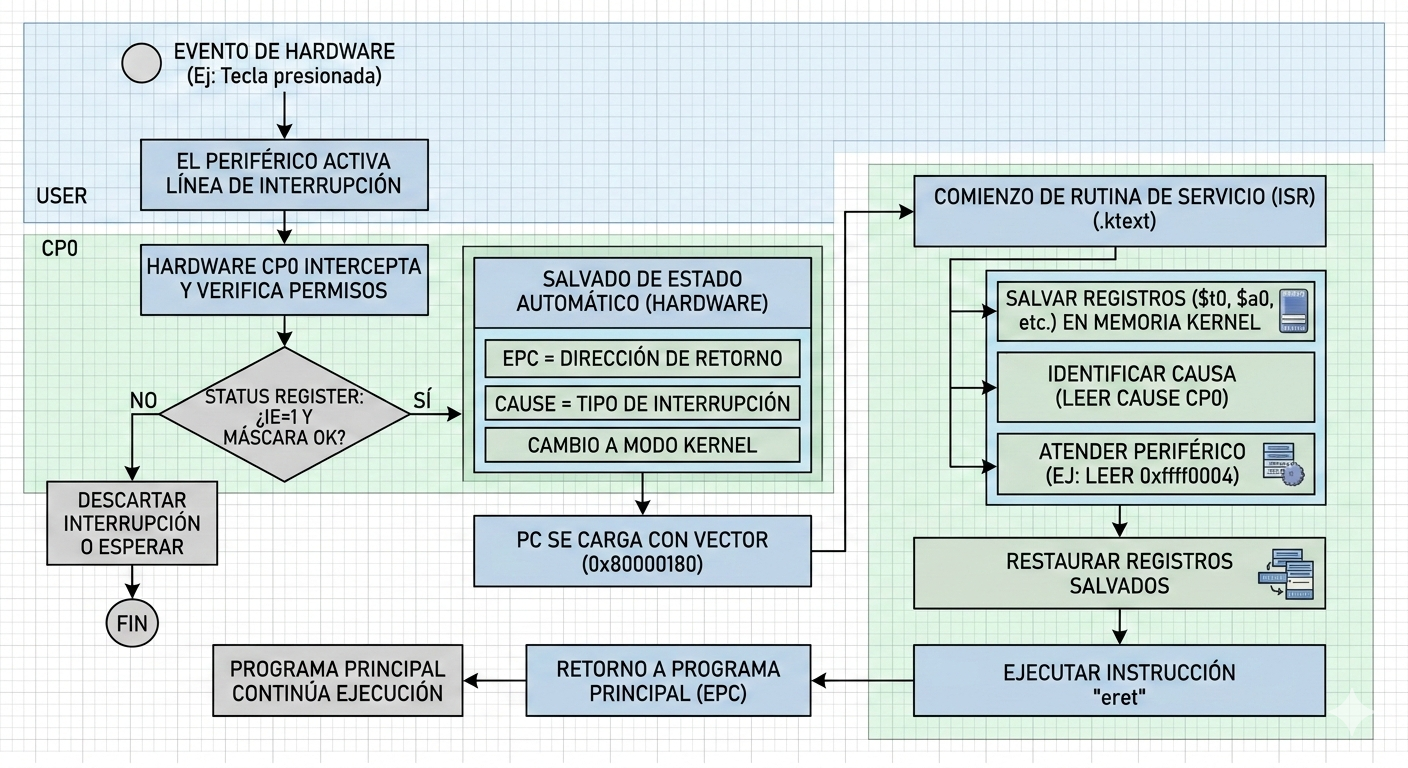
\includegraphics[width=1\textwidth]{diagrama.png} % Ajusta el ancho
		\caption{Diagrama del funcionamiento de la interrupción }
		\label{fig:imagen1}
	\end{figure}
	
\section{Diferencias hay entre gestionar E/S con sondeo y con interrupciones}
	La diferencia fundamental radica en quién tiene el control y cómo se desperdician (o aprovechan) los ciclos de reloj.
	\\\\
	Tabla Comparativa: Sondeo (Polling) vs. Interrupciones\\
	% TODO: \usepackage{array} required
	\begin{tabular}{|>{\centering\arraybackslash}m{4cm}|>{\centering\arraybackslash}m{4cm}|>{\centering\arraybackslash}m{4cm}|}
		\hline
		Característica & Gestión por Sondeo & Gestión por Interrupciones \\
		\hline
		Iniciativa & El CPU pregunta al periférico & El Periférico avisa al CPU \\
		\hline
		Eficiencia & Baja. El CPU pierde tiempo en bucles de espera & Alta. El CPU solo actúa cuando es necesario \\
		\hline
		Determinismo & Muy predecible (sabes cuándo preguntas) & Asíncrono (ocurre en cualquier momento) \\
		\hline
		Complejidad & Muy simple de programar & Compleja (requiere manejar registros del CP0) \\
		\hline
		Carga de Trabajo & Constante, incluso si no hay datos & Proporcional a la actividad del periférico \\
		\hline
	\end{tabular}
	
\section{Ventajas del uso de interrupciones en términos de uso del procesador}
	\begin{enumerate}
		\item \textbf{Uso de la CPU (El concepto de Espera Activa)}\\
			En el sondeo, el programa entra en un bucle llamado espera activa. En cambio, con interrupciones, la CPU sigue ejecutando otras tareas útiles. Cuando el periférico está listo, le envía una señal eléctrica al procesador para que ''atienda la puerta'' solo en ese momento.
		\item \textbf{Latencia de Respuesta}
			\begin{itemize}
				\item \textbf{Sondeo:} Si el CPU está haciendo un cálculo largo entre una pregunta y otra, puede que el dato llegue y tenga que esperar a que el ciclo de sondeo vuelva a pasar por ahí.
				\item \textbf{Interrupciones:} La respuesta es casi inmediata. El hardware fuerza el salto a la rutina de servicio (ISR) en cuanto se activa la línea de interrupción, minimizando el tiempo de respuesta
			\end{itemize}
		\item \textbf{Cuándo usar cada una}
			\begin{itemize}
				\item \textbf{Sondeo:} Es útil en sistemas embebidos muy simples donde el CPU no tiene más tareas que hacer, o cuando el periférico es extremadamente rápido (más rápido que el tiempo que tarda el CPU en gestionar el contexto de una interrupción).
				\item \textbf{Interrupciones:} Es el estándar en sistemas modernos y multitarea (como MARS simula un sistema real), permitiendo que el teclado, el disco duro y el reloj funcionen simultáneamente sin bloquear el sistema.
			\end{itemize}
		
	\end{enumerate}
	
\section{Registros especiales en Mips32 para la gestión de interrupciones}
	Para gestionar interrupciones y excepciones en MIPS32, no se usa los registros de propósito general ($s0, $t0, etc.), sino que se recurre al Coprocesador 0 (CP0). Este es un procesador auxiliar dedicado exclusivamente a las tareas de control del sistema.
	\begin{enumerate}
		\item \textbf{Registros del Coprocesador 0 (CP0)}\\
			\begin{tabular}{|>{\centering\arraybackslash}m{3cm}|>{\centering\arraybackslash}m{7cm}|}
				\hline
				Registro & Función Principal \\
				\hline
				\$12 (Status) & Habilita/Deshabilita las interrupciones. Decide qué periféricos pueden interrumpir y el bit global de habilitación (\$IE\$) \\
				\hline
				\$13 (Cause) & Indica qué pasó. Si ocurre una interrupción, este registro guarda un código que te dice si fue por el teclado, por el reloj o por un error de división por cero \\
				\hline
				\$14 (EPC) & Exception Program Counter. Guarda la dirección de la instrucción que se estaba ejecutando justo antes de que llegara la interrupción \\
				\hline
				\$8 (BadVAddr) & Almacena la dirección de memoria que causó un error \\
				\hline
			\end{tabular}
		\item \textbf{Registros de Periféricos (Memory-Mapped I/O)}\\
			En MIPS, los periféricos se manejan como si fueran direcciones de memoria. Para el teclado y la consola en MARS, los registros clave son:
			\begin{itemize}
				\item \textbf{Keyboard Receiver Control (0xffff0000):}\\
					\begin{itemize}
						\item Bit 0: Ready bit (1 si hay una tecla lista).
						\item Bit 1: Interrupt Enable (Si lo pones en 1, el teclado generará una interrupción cada vez que se presione una tecla).
					\end{itemize}
				\item \textbf{Keyboard Receiver Data (0xffff0004):}\\
					\begin{itemize}
						\item Contiene el código ASCII de la tecla presionada.
					\end{itemize}
			\end{itemize}
	\end{enumerate}
	
\section{¿Por qué es necesario guardar el contexto al entrar en una rutina de servicio?}
	La respuesta corta es: para que el programa principal no se dé cuenta de que fue interrumpido.
	\begin{enumerate}
		\item \textbf{La Transparencia para el Usuario}\\
			El programa que se está ejecutando en el ''User Space'' no sabe que una interrupción va a ocurrir; es un evento asíncrono. Si la rutina de servicio (ISR) utiliza el registro \$t0 para procesar una tecla, y el programa principal también estaba usando \$t0 para un bucle, el valor original se perderá. Al restaurar el contexto, se garantiza que el programa principal continúe exactamente desde el estado en que quedó.
		\item \textbf{Uso de Registros Compartidos}\\
			En MIPS, solo hay 32 registros de propósito general. Tanto el código de usuario como el código del Kernel (la ISR) comparten físicamente los mismos registros.
			\begin{itemize}
				\item Si la ISR no guarda los valores, causará un ''efecto secundario'' (side effect) que corromperá los datos del usuario, provocando errores imposibles de depurar (el programa fallará aleatoriamente dependiendo de cuándo ocurra la interrupción).
			\end{itemize}
		\item \textbf{El Protocolo en MIPS}\\
			A diferencia de una función normal donde usa la pila (\$sp), en una ISR de MARS se suele usar una zona de memoria fija en el segmento de datos del Kernel o los registros reservados \$k0 y \$k1.
	\end{enumerate}
	
\section{Momentos en que pueden generarse excepciones en un sistema MIPS32}
	Es importante diferenciar primero que, aunque a veces usamos excepción e interrupción como sinónimos, en MIPS una interrupción es un evento externo (hardware), mientras que una excepción suele ser un evento interno provocado por la propia ejecución de las instrucciones.
	\subsection{Situaciones en las que se pueda generar una excepción}
		En MIPS32, el registro Cause del Coprocesador 0 identificará el motivo mediante un código específico.
		\begin{enumerate}
			\item \textbf{Desbordamiento Aritmético}\\
				operación con signo (como add o addi) excede el rango representable de 32 bits. Instrucciones como addu ignoran esto, pero add lanza una excepción.
			\item \textbf{Fallo de Dirección}\\
				Se genera cuando se intenta acceder a una dirección de memoria no alineada (por ejemplo, cargar una palabra lw desde una dirección que no es múltiplo de 4) o cuando un programa de usuario intenta acceder al espacio de memoria del Kernel.
			\item \textbf{Instrucción No Válida}\\
				El procesador encuentra un código de operación (opcode) que no reconoce o que no está implementado en su arquitectura.
			\item \textbf{Llamada al Sistema} \\    
				Syscall se usa para solicitar servicios al SO (imprimir en consola, leer teclado) y break es utilizada por los depuradores para detener la ejecución.
		\end{enumerate}
	\subsection{Etapas del pipeline pueden provocar una excepción}
		En un procesador segmentado (pipeline) de 5 etapas, las excepciones pueden surgir en distintos puntos dependiendo de qué parte del hardware detecte el error.
		\\
		\begin{tabular}{|>{\centering\arraybackslash}m{2cm}|>{\centering\arraybackslash}m{9cm}|}
			\hline
			Etapa del Pipeline & ¿Por qué puede ocurrir una excepción? \\
			\hline
			IF & Fallo de acceso a memoria: Si el PC apunta a una dirección inválida o fuera de los límites permitidos para buscar la siguiente instrucción \\
			\hline
			ID & Instrucción ilegal: Aquí es donde la unidad de control se da cuenta de que el opcode no existe o es una instrucción privilegiada en modo usuario \\
			\hline
			EX & Errores aritméticos: Aquí se realizan los cálculos en la ALU. Si hay un overflow, esta etapa levanta la bandera de excepción \\
			\hline
			MEM & Errores de datos: Al intentar un lw o sw. Puede ocurrir por alineación incorrecta (Address Error) o por intentar escribir en una zona de solo lectura \\
			\hline
			WB & Generalmente no genera excepciones nuevas, pero es el punto donde el procesador decide si confirma la excepción ocurrida en etapas previas antes de escribir en el banco de registros \\
			\hline
		\end{tabular}
		
\section{Estrategias de tratamiento de excepciones e interrupciones}
	Aunque a menudo se usan como sinónimos en conversaciones informales, para un arquitecto de computadores son eventos con naturalezas opuestas.
	\subsection{Diferencias entre interrupciones y excepciones}
		\begin{tabular}{|>{\centering\arraybackslash}m{2.5cm}|>{\centering\arraybackslash}m{4cm}|>{\centering\arraybackslash}m{4cm}|}
			\hline
			Característica & Interrupciones & Interrupciones \\
			\hline
			Característica & Externo: Periféricos (teclado, disco, reloj) & Interno: La propia ejecución de una instrucción \\
			\hline
			Sincronía & Asíncronas: Pueden ocurrir en cualquier momento, sin importar qué instrucción se esté ejecutando & Síncronas: Ocurren en una instrucción específica (ej. al dividir por cero o al ejecutar un syscall) \\
			\hline
			Predictibilidad & Impredecibles. El programador no sabe cuándo llegará el dato & Reproducibles. Si ejecuta el mismo código con los mismos datos, fallará en el mismo punto \\
			\hline
		\end{tabular}
	\subsection{Estrategias de tratamiento en MIPS32}
		Existen dos formas principales en las que un procesador puede organizar cómo responder a estos eventos:
		\begin{enumerate}
			\item \textbf{Vectorización}\\
				En esta estrategia, cada tipo de evento tiene una dirección de memoria única asignada. El hardware salta directamente a la dirección específica según la causa.
				\begin{itemize}
					\item \textbf{Ventaja:} Es más rápido porque no hay que ''preguntar'', el salto ya lo dice.
				\end{itemize}
			\item \textbf{Manejador Único}\\
				Es la estrategia que utiliza MIPS32 y MARS. Todas las excepciones e interrupciones saltan a la misma dirección de memoria (usualmente 0x80000180).
				\begin{itemize}
					\item \textbf{¿Cómo se redirige?} Una vez en esa dirección, el software debe leer el registro Cause del Coprocesador 0. Mediante una estructura de control (como un if-else o un switch), el código identifica el código de excepción (ExcCode) y salta a la subrutina correspondiente.
				\end{itemize}
		\subsubsection{Función del registro EPC}
			El EPC es el marcador del procesador. Cuando ocurre una interrupción o excepción, el hardware guarda automáticamente en el EPC la dirección de la instrucción que se estaba ejecutando o la que le seguía.
			\begin{itemize}
				\item \textbf{Su función vital:} Sin el EPC, el procesador ''olvidaría'' dónde estaba antes de ser interrumpido.
				\item \textbf{El retorno:} Al final de la rutina de servicio, la instrucción eret toma el valor guardado en el EPC y lo carga de vuelta en el Program Counter, permitiendo que el programa de usuario continúe exactamente donde se quedó.
			\end{itemize}
			En el caso de excepciones por error (como un overflow), el EPC apunta a la instrucción que falló para que el sistema operativo pueda decidir si terminar el programa o intentar corregirlo.
		
		\end{enumerate}
		
\section{Habilitación de interrupciones en dispositivos y procesador}
	Es fundamental entender que la habilitación de interrupciones funciona como una serie de interruptores en cascada: si uno está apagado, la señal no llega al destino final.
	
	\subsection{Cómo habilitar las interrupciones}
		\begin{enumerate}
			\item \textbf{En el Teclado (Receiver)}\\
				El teclado se controla mediante el Receiver Control Register en la dirección 0xffff0000.
				\begin{itemize}
					\item \textbf{Procedimiento:} Debe poner en 1 el bit 1 (Interrupt Enable bit) de este registro.
				\end{itemize}
			\item \textbf{En la Pantalla (Transmitter)}\\
				La pantalla (consola) funciona de forma similar mediante el Transmitter Control Register en la dirección 0xffff0008.
				\begin{itemize}
					\item \textbf{Procedimiento:} Se debe poner en 1 el bit 1 de dicha dirección. Esto hará que el hardware genere una interrupción cada vez que la pantalla esté lista para mostrar un nuevo carácter.
				\end{itemize}
			\item \textbf{En el Procesador (Registro Status)}\\
				Aquí es donde el Coprocesador 0 (CP0) decide si acepta o ignora las señales que vienen de afuera. Debe modificar el registro \$12 (Status):
				\begin{itemize}
					\item \textbf{Bit 0 (IE - Interrupt Enable):} Es el interruptor maestro. Si es 0, no entra nada. Debe estar en 1
					\item \textbf{Bits 8-15 (Interrupt Mask):} Cada bit corresponde a un nivel de interrupción (teclado, reloj, etc.). Generalmente, para habilitar las interrupciones de los periféricos en MARS, se activan los bits del 8 al 15 (poniéndolos en 1).
				\end{itemize}
		\end{enumerate}
	\subsection{¿Qué pasaría si habilitamos los dispositivos pero NO el procesador?}
		Si se activa el bit de interrupción en el teclado (0xffff0000) pero se deja el bit IE del registro Status en 0, ocurriría lo siguiente:
		\begin{enumerate}
			\item \textbf{Silencio Administrativo:} El periférico (teclado) efectivamente enviará la señal eléctrica de interrupción hacia el procesador cada vez que se presione una tecla.
			\item \textbf{Bloqueo en el CP0:} El hardware del Coprocesador 0 recibirá la señal, pero al ver que su ''interruptor maestro'' (Status Bit 0) está apagado, ignorará la petición.
			\item \textbf{Resultado en el programa:} El programa principal seguirá ejecutándose normalmente sin saltar nunca a la Rutina de Servicio (ISR). Los datos del teclado se quedarán esperando en el registro de datos (0xffff0004), pero nadie avisará al software de que están ahí.
		\end{enumerate}
		
\section{Procesamiento de interrupciones}
	\subsection{Ciclo de una Interrupción de Reloj Paso a Paso}
		\begin{enumerate}
			\item \textbf{El Evento (Hardware)}\\
				El temporizador interno del sistema alcanza el valor programado. Envía una señal eléctrica al procesador indicando que el tiempo ha expirado.
			\item \textbf{Respuesta Automática (Hardware)}\\
				Antes de que el software haga nada, el hardware de MIPS32 realiza lo siguiente:
				\begin{itemize}
					\item \textbf{Congela la ejecución:} Detiene el programa actual al finalizar la instrucción en curso.
					\item \textbf{Salva el retorno:} Copia la dirección de la siguiente instrucción en el registro EPC.
					\item \textbf{Registra la causa:} Escribe el código correspondiente a ''Interrupción de Hardware'' en el registro Cause.
					\item \textbf{Cambio de estado:} Deshabilita otras interrupciones (pone $IE=0$ en Status) y entra en modo Kernel.
					\item \textbf{Salto:} Carga el PC con la dirección 0x80000180.
				\end{itemize}
			\item \textbf{Rutina de Servicio (Software)}\\
				Aquí es donde entra el código o el del Sistema Operativo:
				\begin{itemize}
					\item \textbf{Salva el Contexto:} Se guardan los registros en memoria (generalmente en el segmento .kdata o en la pila del kernel).
					\item \textbf{Atención del Servicio:} El software reconoce que fue el reloj (leyendo el registro Cause) e incrementa un contador de tiempo o cambia de proceso.
					\item \textbf{Reinicio del Timer:} Se le indica al periférico de reloj que empiece a contar de nuevo para la próxima interrupción.
				\end{itemize}
			\item \textbf{Finalización y Retorno (Software + Hardware)}\\
				\begin{itemize}
					\item \textbf{Restaura el Contexto:} El software recupera los valores originales de los registros desde la memoria.
					\item \textbf{Instrucción eret:} El software ejecuta eret. El hardware, en respuesta, devuelve el valor del EPC al PC y restaura el bit $IE$ en el registro Status, permitiendo que el programa de usuario continúe y que nuevas interrupciones puedan entrar.
				\end{itemize}
			\textbf{Registros que se guardan y restauran}:\\
			\begin{tabular}{|>{\centering\arraybackslash}m{5cm}|>{\centering\arraybackslash}m{6cm}|}
				\hline
				Tipo & Registros Específicos \\
				\hline
				Registros de Propósito General & Todos los que la ISR vaya a utilizar (mínimo \$at, \$v0, \$a0, \$t0-\$t9). \\
				\hline
				Registros Especiales & \$hi y \$lo (si la ISR hace multiplicaciones o divisiones). \\
				\hline
				Registros de Control (CP0) & El registro Status y, en interrupciones anidadas, el EPC. \\
				\hline
			\end{tabular}
		\end{enumerate}
	\subsection{Importancia de guardar el contexto}
		la ISR simula el funcionamiento de periféricos y gestiona eventos. Si no guardáramos estos tres elementos, el sistema colapsaría por las siguientes razones:
		\begin{enumerate}
			\item \textbf{Registros Generales:} Si el programa de usuario estaba haciendo un cálculo y la ISR usa los mismos registros para contar el tiempo, al volver, el cálculo del usuario tendrá resultados basura. Guardarlos asegura la integridad de los datos.
			\item \textbf{EPC:} Si se pierde el EPC, el procesador no sabe a dónde regresar. Es como cerrar un libro y perder el número de página, el programa de usuario ''moriría'' ahí mismo porque el PC no tendría una dirección válida a la cual volver.
			\item \textbf{Registro Status:} Es vital guardarlo porque contiene el estado de privilegios del procesador y la máscara de interrupciones. Si la ISR cambia el modo de ''Usuario'' a ''Kernel'' y no restaura el registro Status al salir, el programa de usuario podría quedarse con permisos de Kernel (un riesgo de seguridad) o con las interrupciones deshabilitadas permanentemente.
		\end{enumerate}
		Guardar el contexto es lo que permite que la interrupción sea transparente. El programa de usuario no debe pensar que fue detenido y reanudado.

\section{Interrupciones de reloj y control de ejecución}
	Este es el punto donde la teoría se convierte en la base de los Sistemas Operativos modernos. El reloj no es solo para dar la hora, es el ''árbitro'' que decide quién juega y por cuánto tiempo en el procesador
	
	\subsection{Usos de interrupción de reloj}
		En un sistema MIPS32, el temporizador actúa como un monitor de seguridad externo al flujo del programa.
		\begin{enumerate}
			\item \textbf{Evitar bucles infinitos}\\
			Sin interrupciones de reloj, un programa con un error lógico tipo j loop (bucle infinito) tomaría el control total de la CPU y el sistema se ''congelaría''.
			\begin{itemize}
				\item \textbf{Mecanismo:} El Sistema Operativo configura el reloj para que genere una interrupción cada $X$ milisegundos.
				\item \textbf{Acción:} Cuando el reloj interrumpe, el control pasa forzosamente a la Rutina de Servicio (ISR). El procesador deja de ejecutar el bucle infinito para ejecutar el código del Kernel. En ese momento, el Kernel puede detectar que el programa lleva demasiado tiempo sin ceder el control y decidir suspenderlo o terminarlo.
			\end{itemize}
			\item \textbf{Finalizar programas con tiempo máximo}\\
			Esto es muy común en servidores o sistemas de corrección automática (como los que se usan en concursos de programación).
			\begin{itemize}
				\item \textbf{Mecanismo:} Al iniciar el programa, el Kernel guarda en una variable del segmento .kdata el tiempo de inicio y el límite permitido (ej. 5 segundos).
				\item \textbf{Acción:} En cada interrupción de reloj, la ISR incrementa un contador. Si contador > limite, la ISR no ejecuta la instrucción eret para volver al programa de usuario. En su lugar, limpia la memoria y salta a una rutina de finalización de proceso, informando que el tiempo ha expirado.
			\end{itemize}
			
		\end{enumerate}
		
	\subsection{¿Qué pasa si el programa finaliza antes de tiempo?}
		Si el programa de usuario termina su tarea exitosamente antes de que el reloj mande su señal, el software (el programa de usuario) debe realizar una salida ordenada:
		\begin{enumerate}
			\item \textbf{Llamada al Sistema:} 
				El programa debe ejecutar un syscall de salida (en MARS es cargar \$v0 con 10 o 17 y ejecutar syscall).
			\item \textbf{Desactivación del Timer:} Es responsabilidad del Sistema Operativo (o de la rutina de salida) deshabilitar la interrupción de reloj pendiente. Si no se hace, el reloj interrumpirá un proceso que ya no existe o interrumpirá al propio Kernel mientras intenta cargar el siguiente programa.
			\item \textbf{Liberación de Recursos:} Se limpian los registros y se marca ese espacio de tiempo como "disponible" para que el planificador (scheduler) asigne el procesador a otra tarea inmediatamente, sin esperar a que el temporizador llegue a cero.
		\end{enumerate}
		En MARS, cuando se usa el "Timer Tool", se observa que si el programa hace un li \$v0, 10; syscall, la simulación se detiene y las interrupciones pendientes se descartan automáticamente.
		
\section{Análisis y Discusión de los Resultados}
	\begin{enumerate}
		\item \textbf{La Dualidad de la Gestión de E/S: Eficiencia vs. Simplicidad}\\
			A través del desarrollo de la práctica, se observó que la implementación de Sondeo (Polling), aunque mecánicamente más sencilla de codificar, impone una carga ineficiente sobre el procesador. En los algoritmos probados, el CPU permanece en un estado de espera activa, consumiendo ciclos de reloj innecesarios que podrían emplearse en cálculos de segundo plano.
			\\\\
			Por el contrario, la transición hacia un modelo basado en Interrupciones permitió que el sistema operara bajo un esquema de demanda. La importancia de este hallazgo radica en la capacidad de respuesta: mientras que el sondeo puede perder eventos si la ráfaga de datos es más rápida que el ciclo de consulta, la interrupción garantiza que el hardware del Coprocesador 0 (CP0) capture el evento en el instante exacto de su ocurrencia, marcando la diferencia entre un sistema de tiempo real y uno de propósito general limitado.
			
		\item \textbf{El Rol Crítico del Coprocesador 0 (CP0) y la Jerarquía de Control}\\
			Un punto fundamental de discusión es la interacción con los registros especiales. Se determinó que la gestión de excepciones en MIPS32 no es una tarea del set de instrucciones principal, sino una función delegada al CP0.
			\begin{itemize}
				\item El uso de los registros Status (\$12) y Cause (\$13) demostró ser el "mecanismo de filtrado" del procesador.
				\item Se analizó que la habilitación de interrupciones no es un evento único, sino una cadena de permisos: desde el bit de habilitación en el periférico (ej. teclado en 0xffff0000) hasta la máscara de interrupción y el bit global $IE$ en el registro Status.
			\end{itemize}
			Esta estructura jerárquica es vital para la seguridad del sistema, ya que permite al núcleo del sistema operativo priorizar ciertos eventos (como fallos de memoria) sobre otros menos críticos (como la entrada de teclado).
		\item \textbf{Preservación del Contexto: La Invisibilidad del Kernel}\\
			Durante la simulación de interrupciones de reloj y teclado, se evidenció que la transparencia es el objetivo primordial de una Rutina de Servicio (ISR). El análisis del uso de los registros $k0 y $k1 reveló su importancia táctica: son los únicos registros que el programador de nivel de usuario no debe tocar, permitiendo que el Kernel tenga un ''espacio de maniobra'' para salvar el resto del contexto (registros temporales, $v0, $a0, etc.) sin destruir los datos que el programa principal está procesando.
			\\\\
			La discusión sobre el registro EPC (Exception Program Counter) fue central. Se concluyó que el EPC es el único vínculo que permite al procesador regresar de un estado de excepción al flujo normal. Sin una gestión correcta del EPC y la instrucción eret, el sistema entraría en un estado de inconsistencia o "pánico de núcleo".
			
		\item \textbf{Control de Ejecución y Determinismo}\\
			Finalmente, la implementación de interrupciones de reloj permitió discutir el concepto de multitarea cooperativa vs. apropiativa. Se demostró que el reloj funciona como un "vigilante" (Watchdog), capaz de romper bucles infinitos y garantizar que ningún proceso monopolice la CPU. Esto transforma al procesador MIPS32 de una simple calculadora secuencial en una plataforma capaz de gestionar un entorno de ejecución controlado y seguro, simulando de manera efectiva el comportamiento de un sistema operativo moderno.
	\end{enumerate}
	La práctica permitió validar que la arquitectura MIPS32, mediante su sistema de excepciones e interrupciones, ofrece un marco robusto para la interacción con el mundo exterior. La comprensión del manejo de registros en el CP0 y la preservación del contexto no solo son ejercicios de programación, sino la base fundamental sobre la cual se construyen la estabilidad y la concurrencia en los sistemas de computación actuales.

\end{document}
